\providecommand{\main}{../../../..}
\documentclass[\main/dresen_thesis.tex]{subfiles}
\begin{document}
  \label{sec:looselyPackedNS:bilayerStacks:gisaxs}
  \begin{figure}[tb]
    \centering
    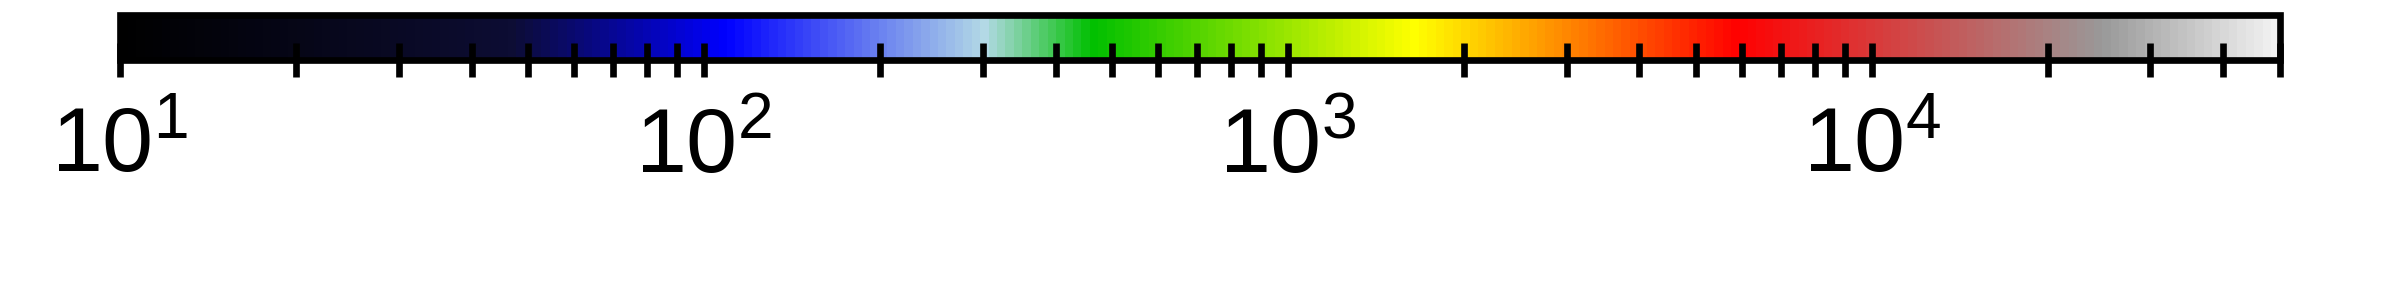
\includegraphics{looselyPackedNP_8BL-IOS-11_GISAXS_SVcbar}
    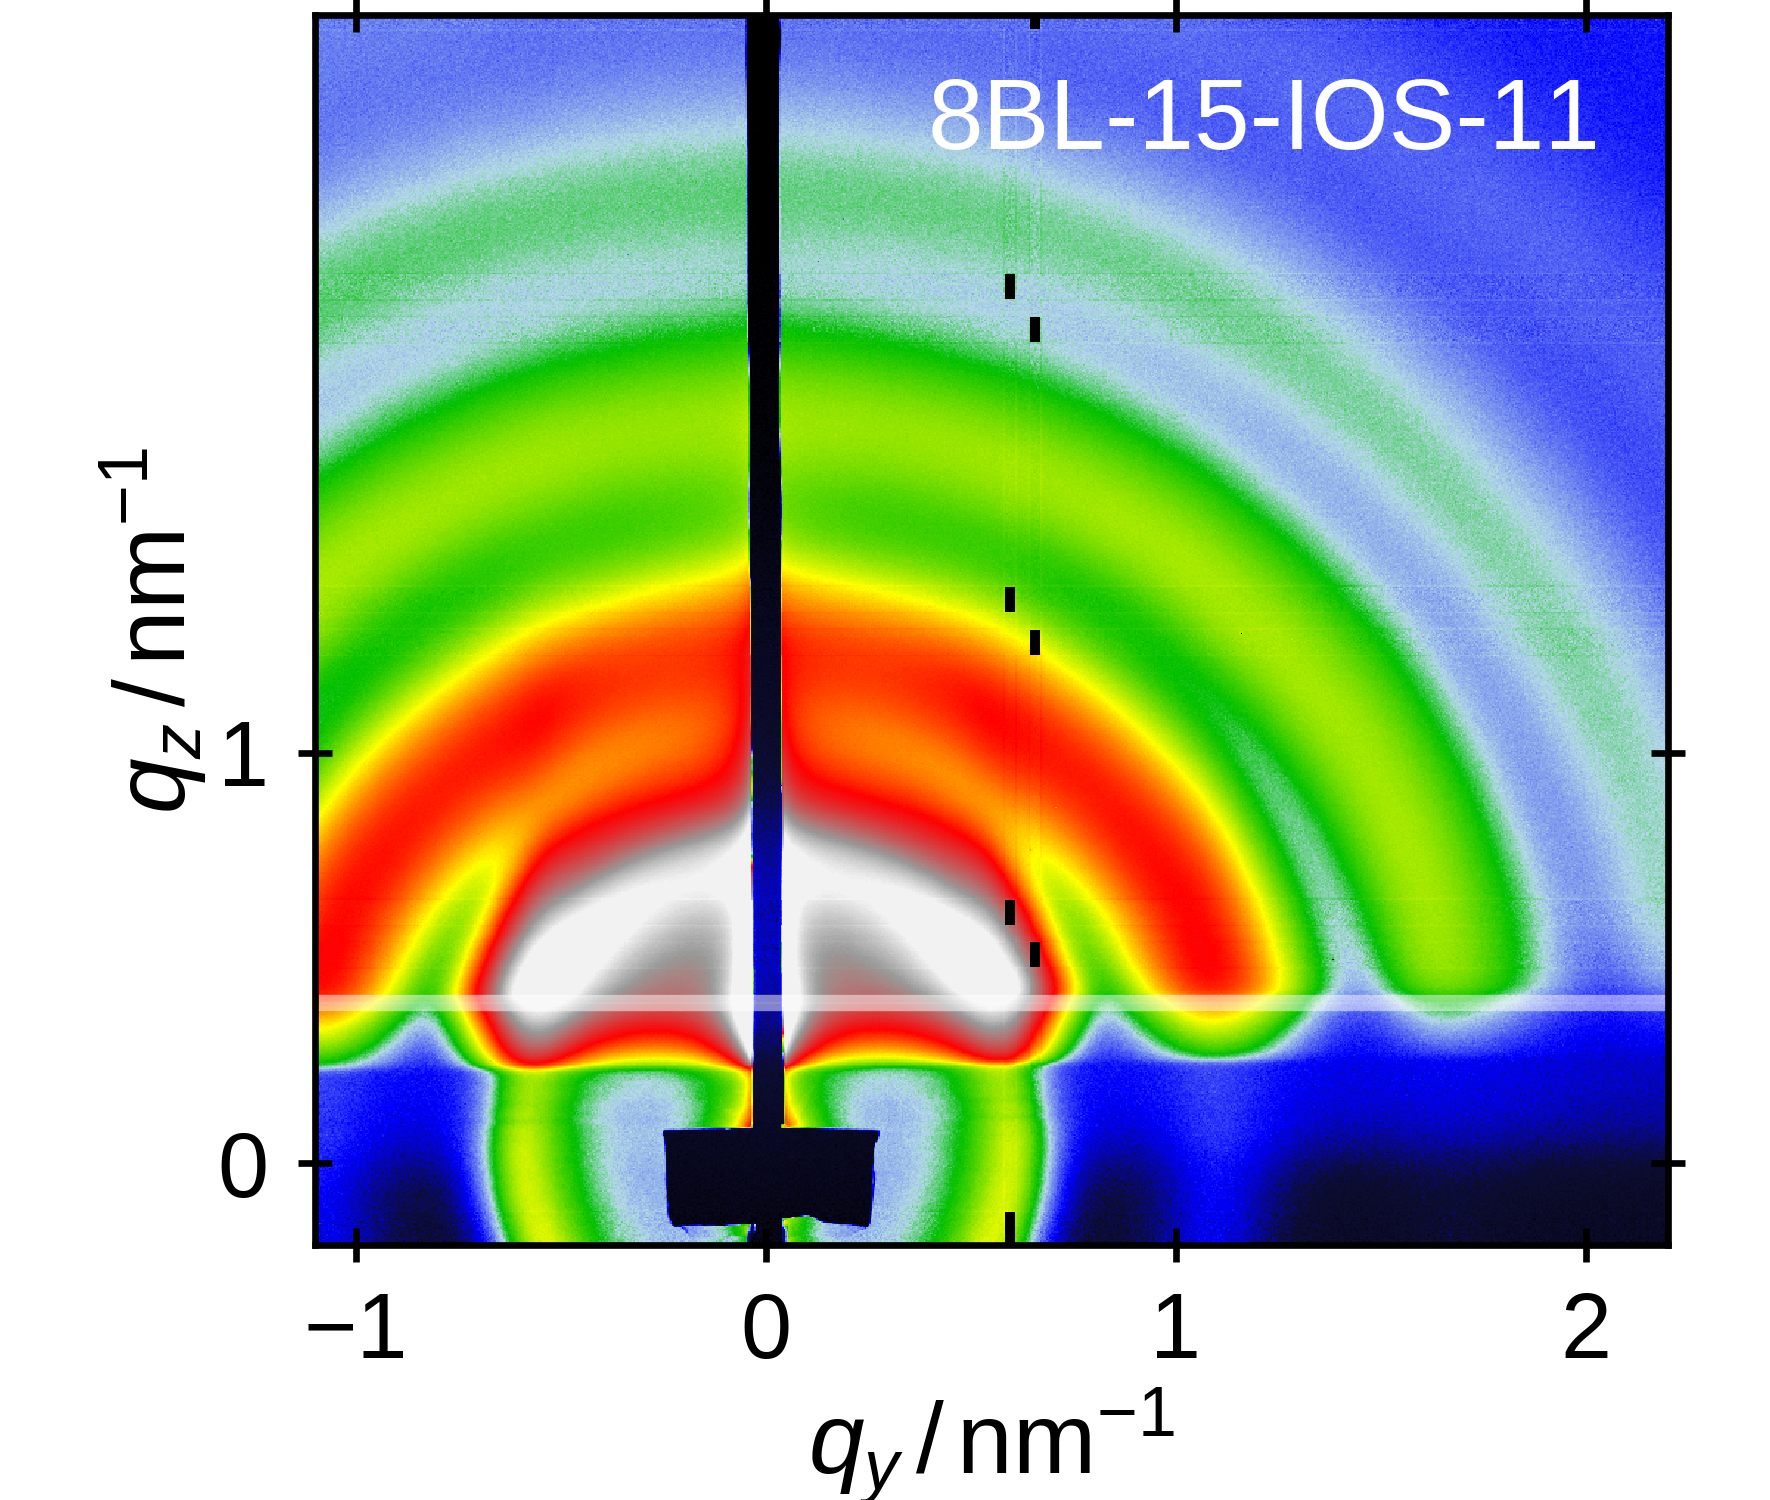
\includegraphics{looselyPackedNP_GISAXS_8BL-15-IOS-11}
    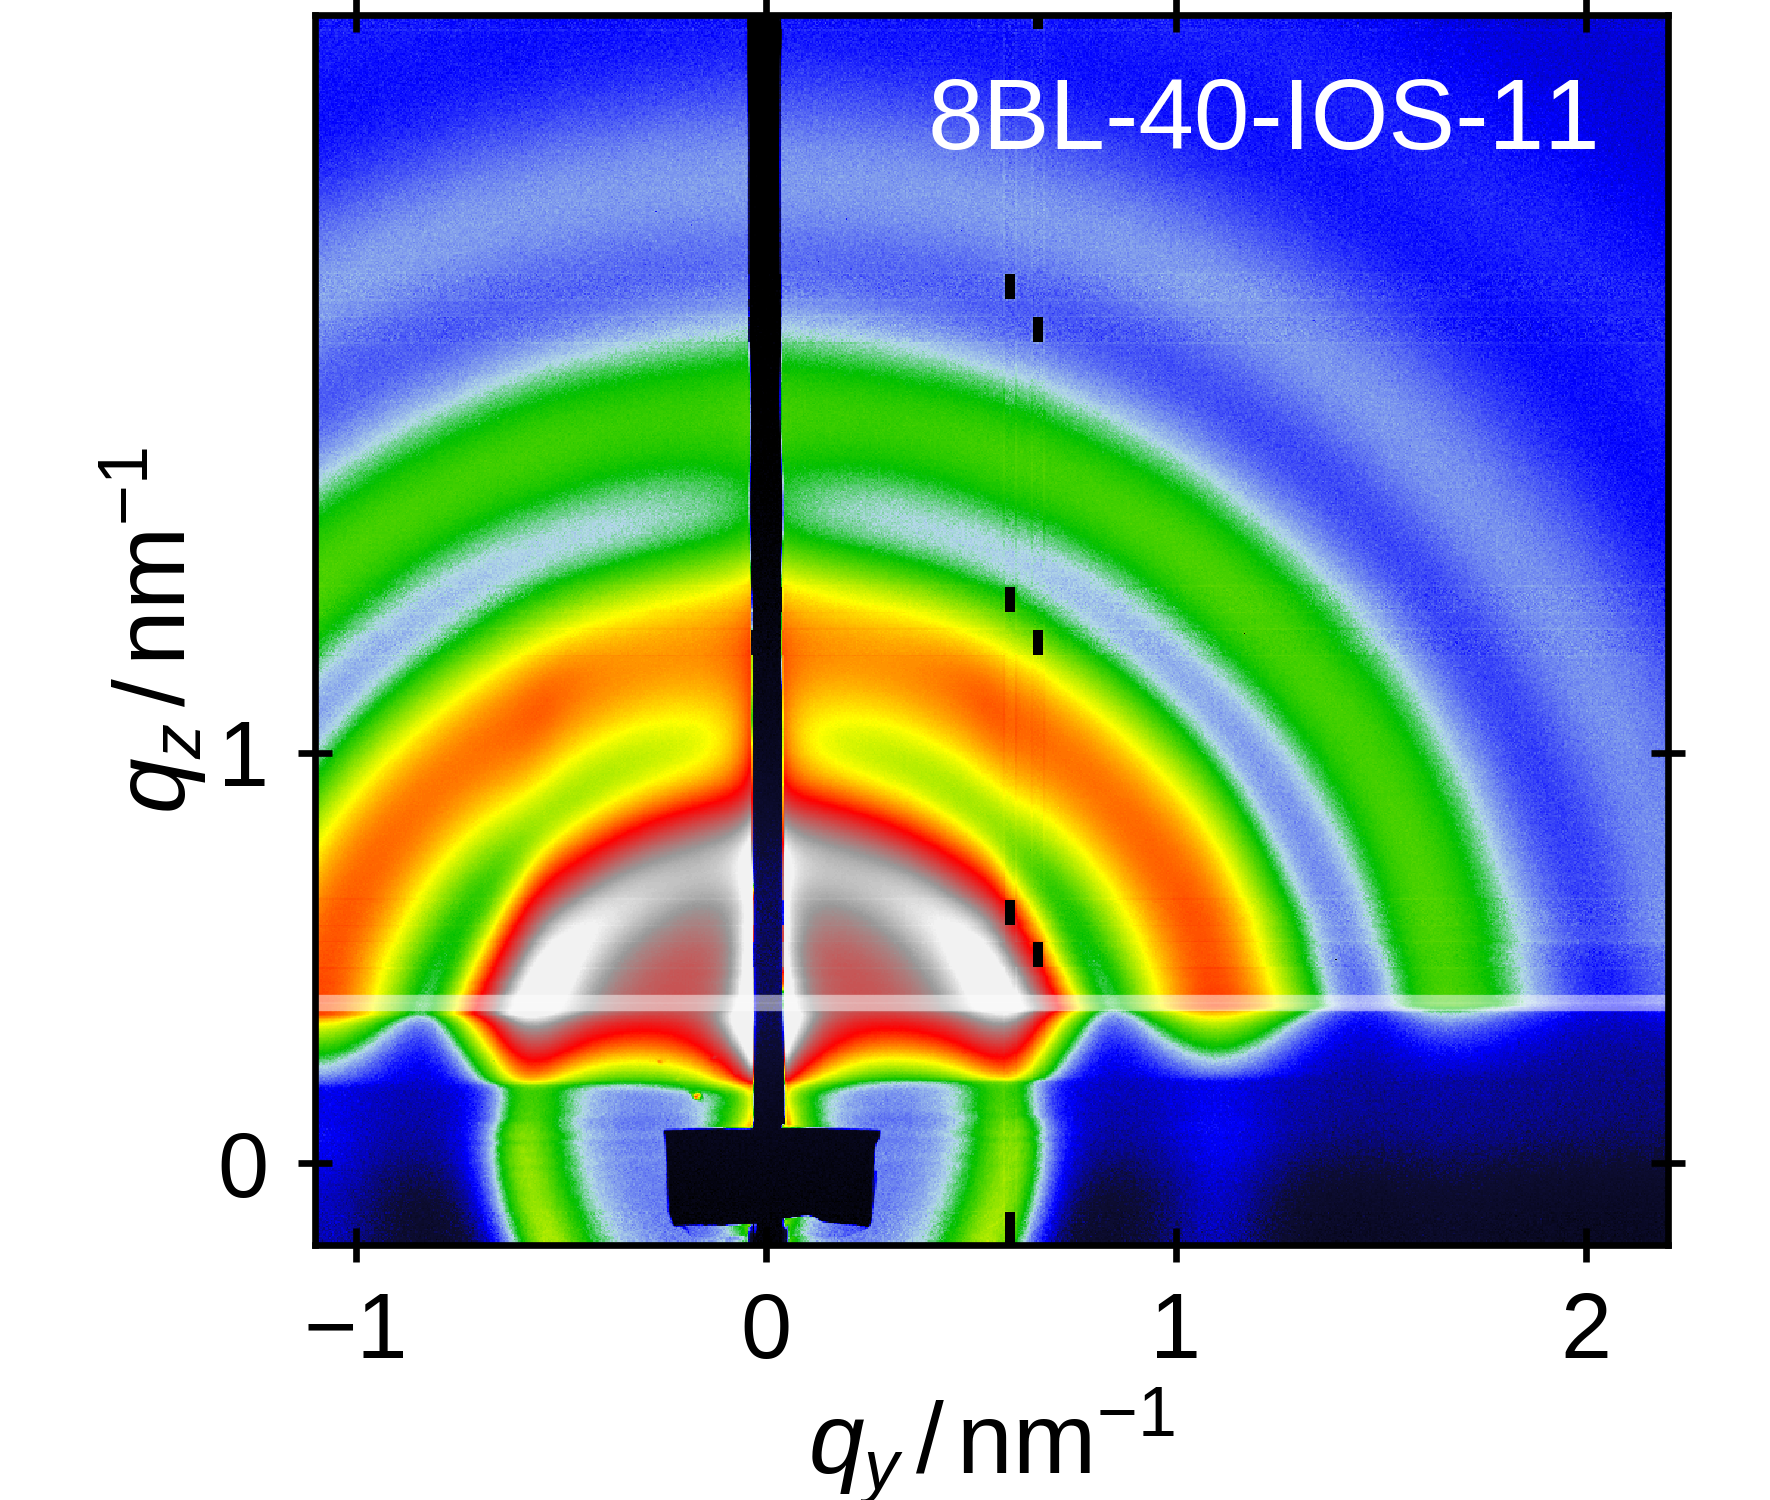
\includegraphics{looselyPackedNP_GISAXS_8BL-40-IOS-11}
    \caption{\label{fig:looselyPackedNP:bilayerStacks:gisaxs8BL_IOS_11}GISAXS detector images of 8BL-15-IOS-11 (left)  and 8BL-40-IOS-11 (right) measured at BM26B under an incident angle of $\alpha_i \eq 0.2 ^\circ$.}
  \end{figure}

  \begin{figure}[tb]
    \centering
    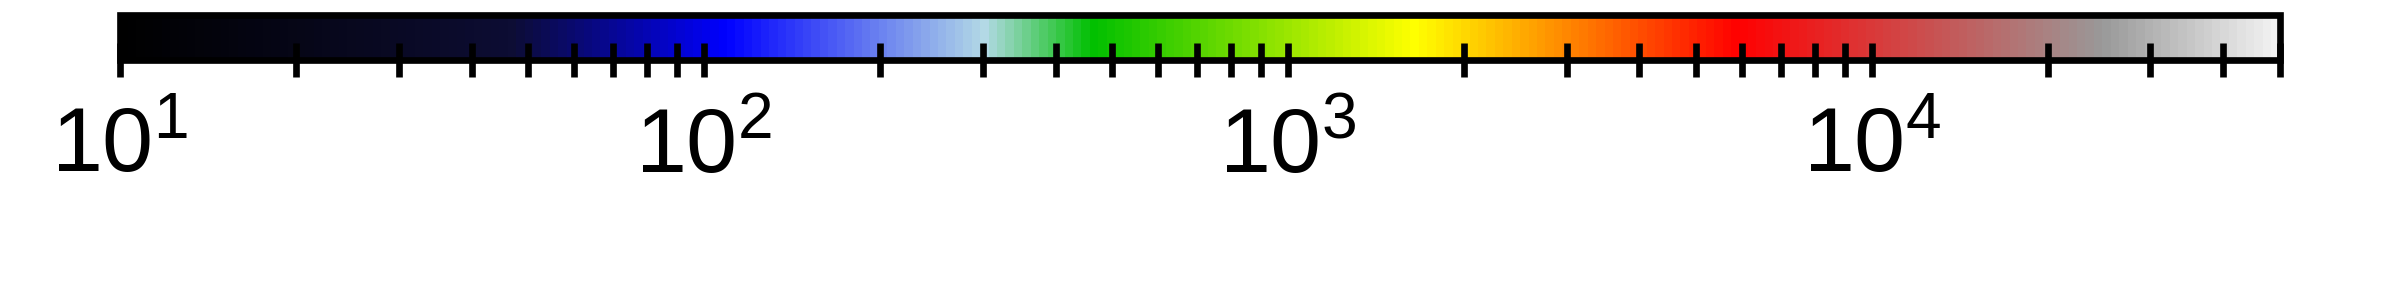
\includegraphics{looselyPackedNP_8BL-IOS-7_GISAXS_SVcbar}
    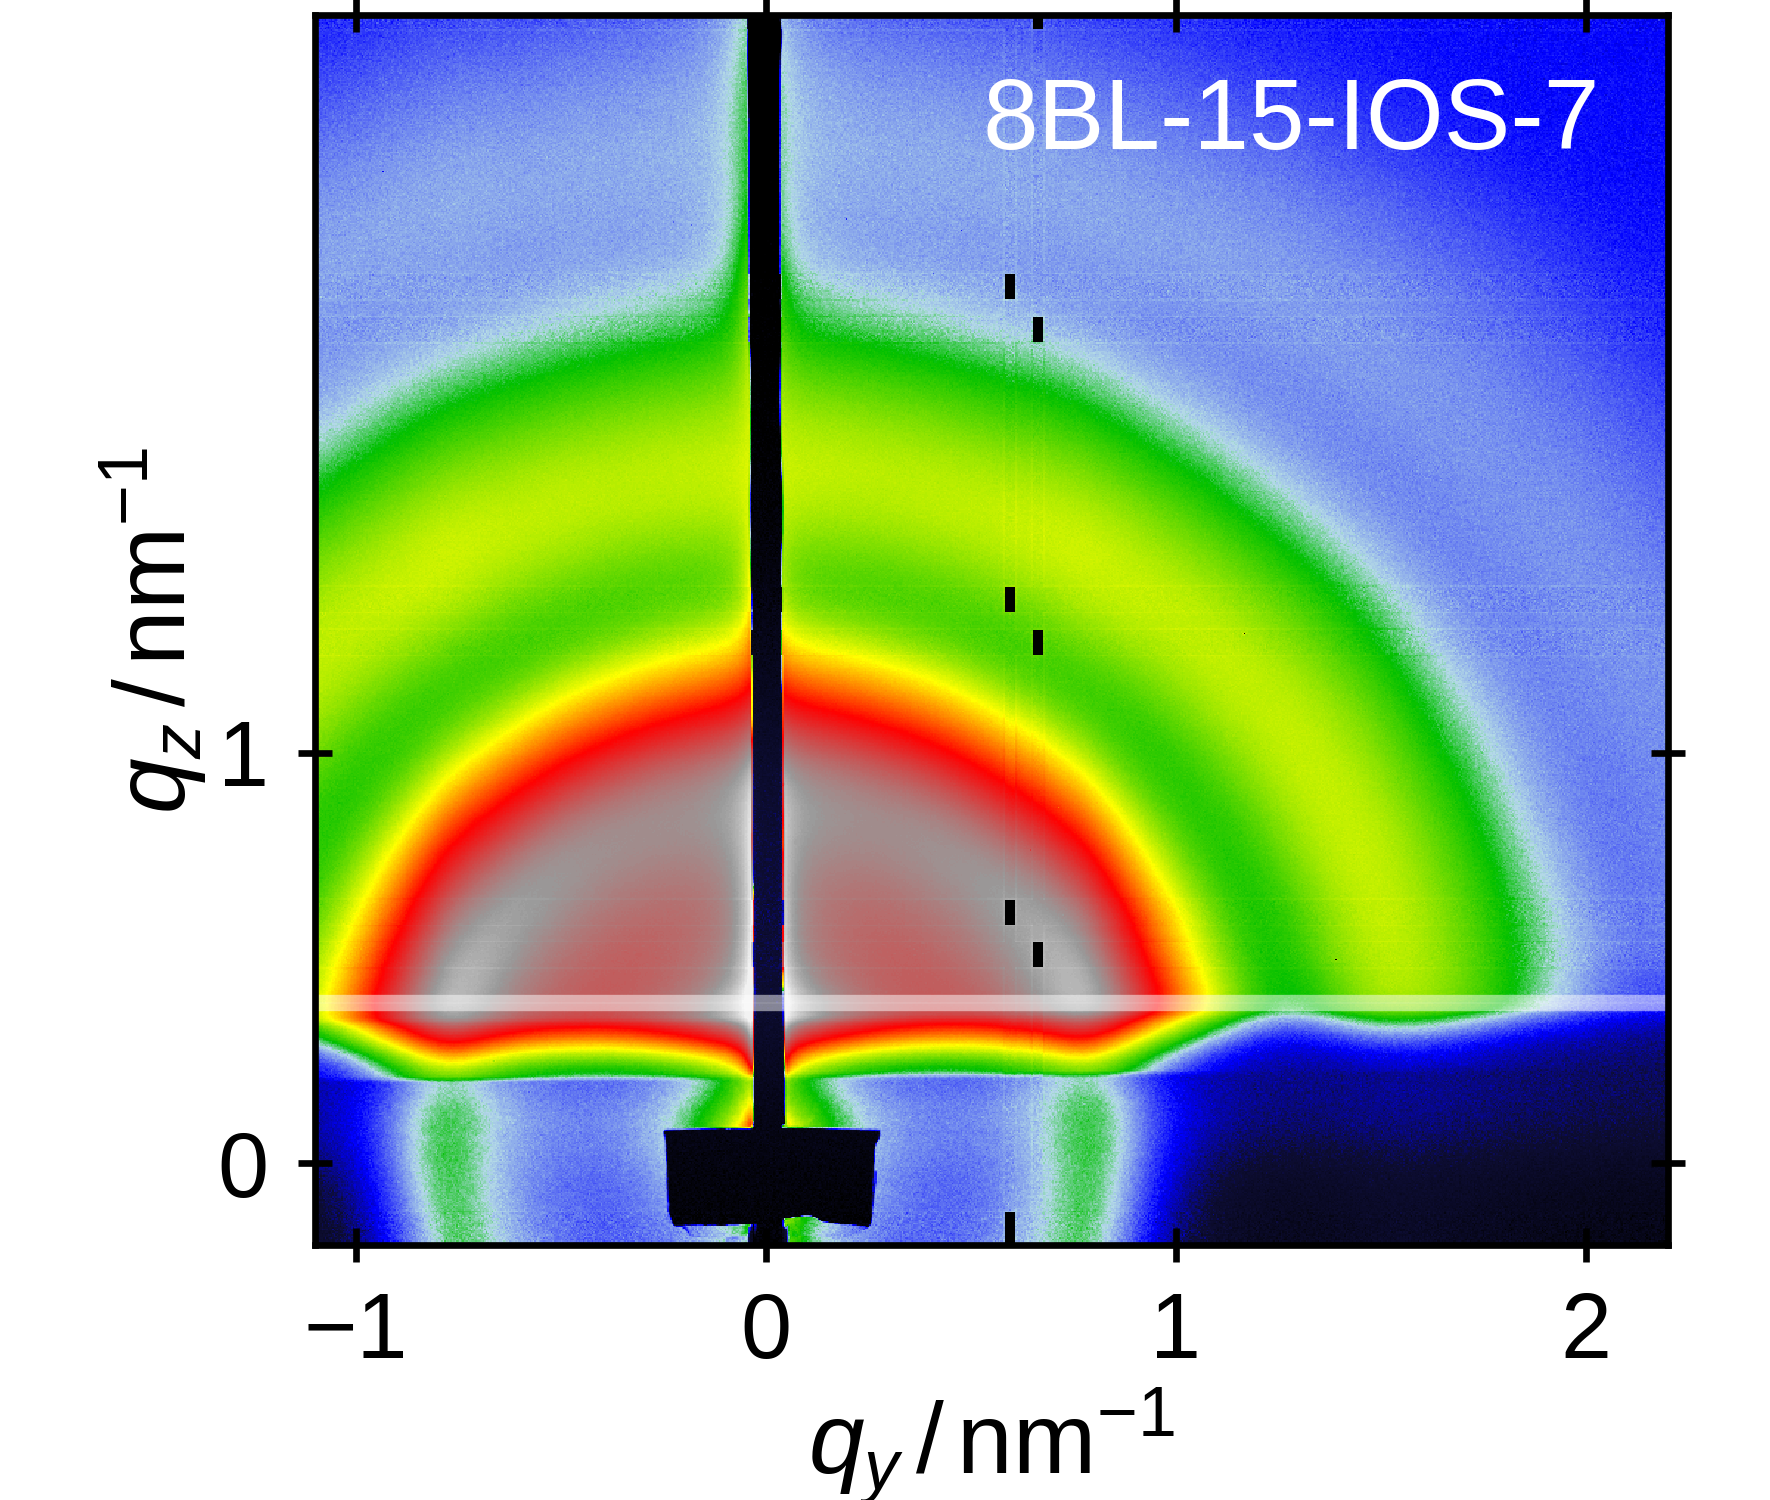
\includegraphics{looselyPackedNP_GISAXS_8BL-15-IOS-7}
    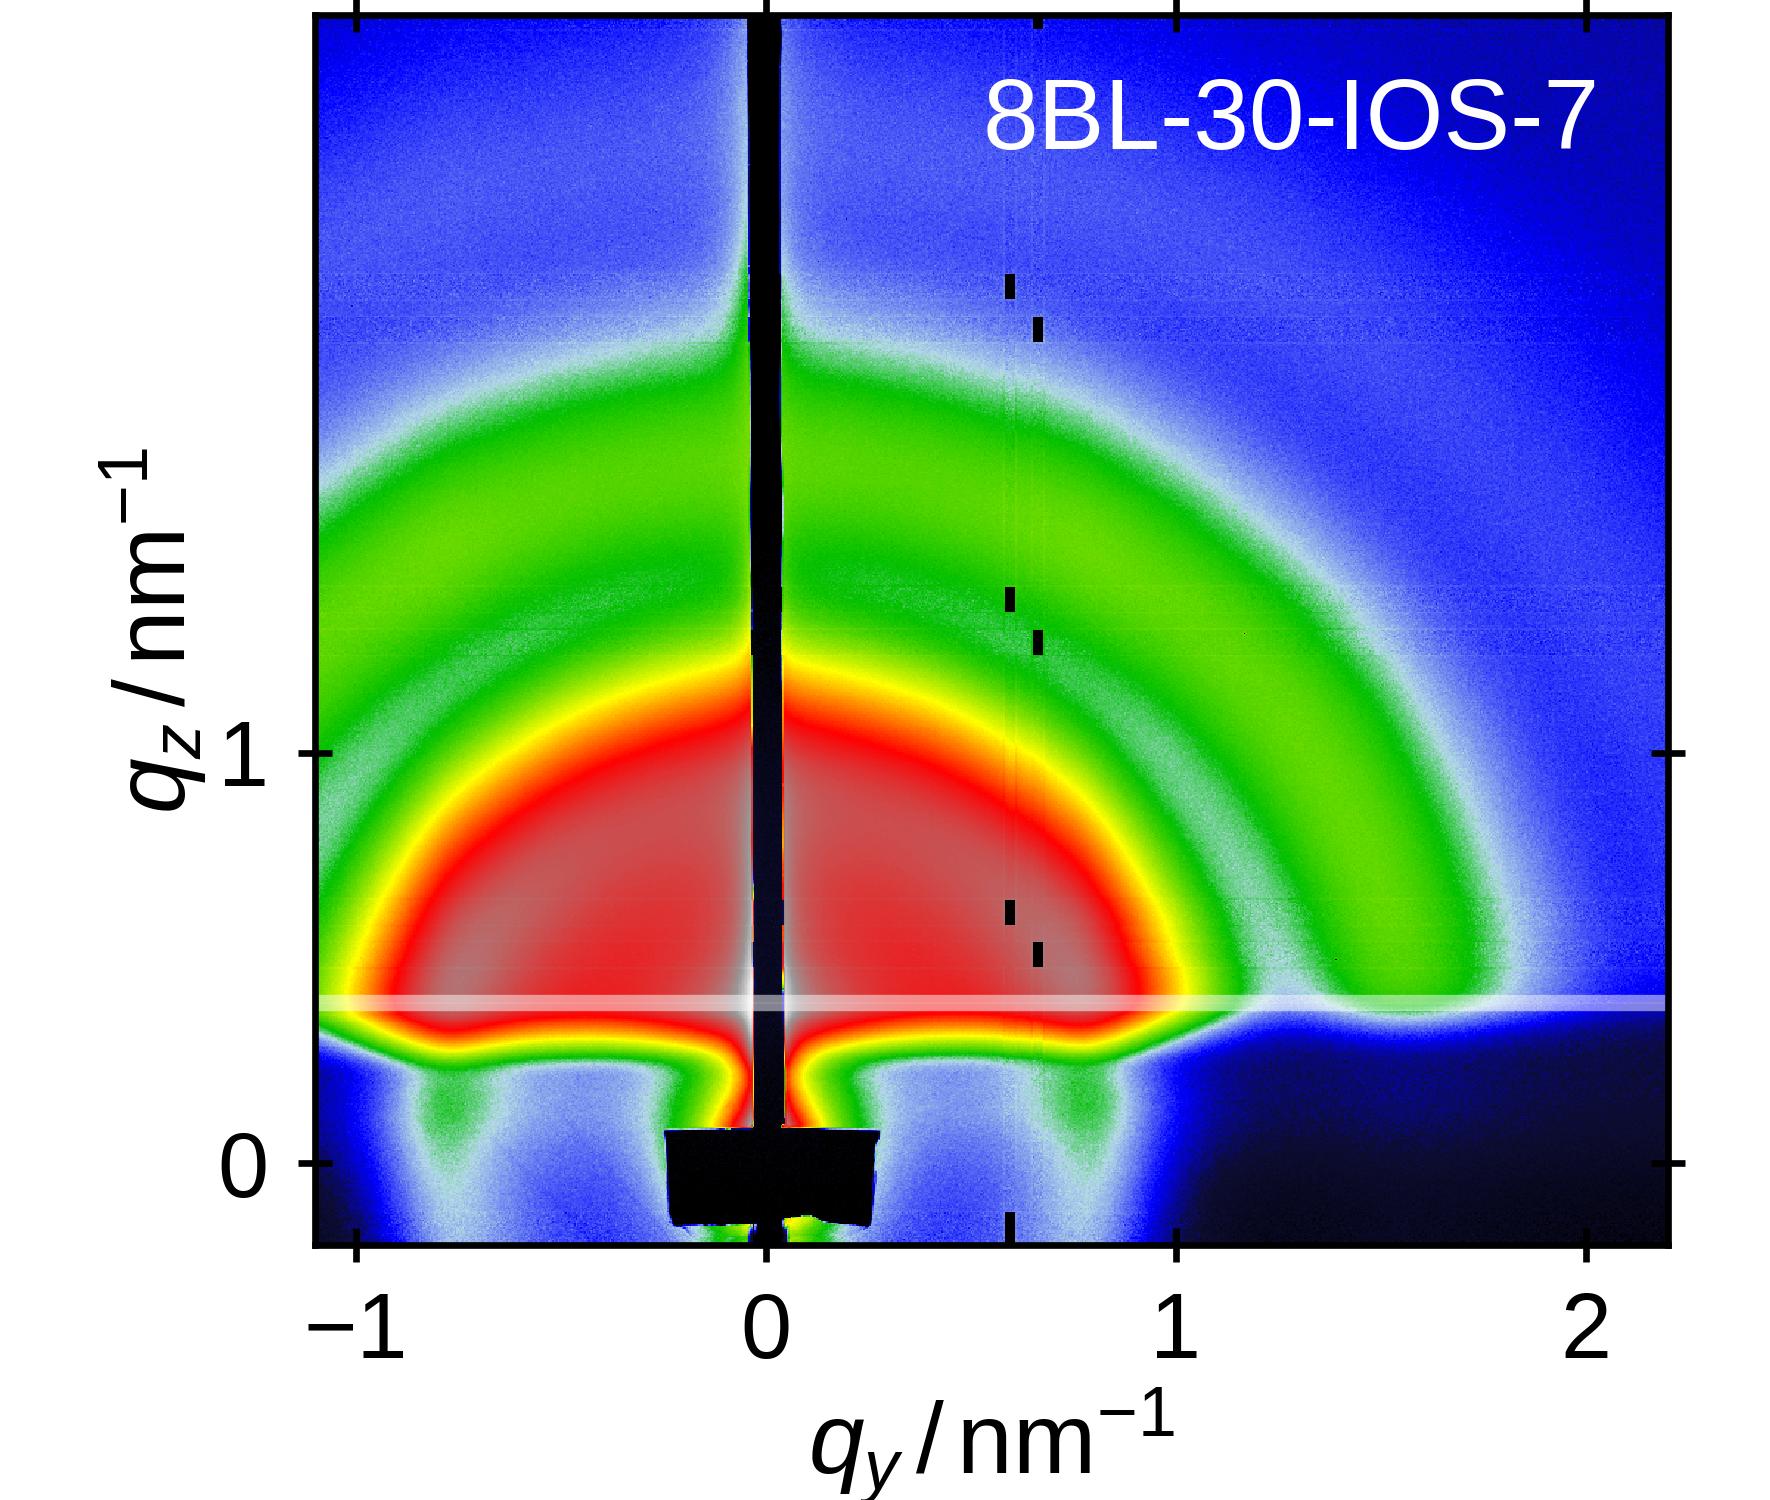
\includegraphics{looselyPackedNP_GISAXS_8BL-30-IOS-7}
    \caption{\label{fig:looselyPackedNP:bilayerStacks:gisaxs8BL_IOS_7}GISAXS detector images of 8BL-15-IOS-7 (left)  and 8BL-30-IOS-7 (right) measured at BM26B under an incident angle of $\alpha_i \eq 0.2 ^\circ$.}
  \end{figure}

  The four bilayer stacks are studied by grazing-incidence X-ray scattering, with the measurement having been performed at the BM26B beamline (\refsec{ch:lss:BM26B}) at the ESRF.
  The detector images obtained at the large sample-to-detector distance under an incident angle of $0.2 ^\circ$ for the samples from IOS-11 are shown in \reffig{fig:looselyPackedNP:bilayerStacks:gisaxs8BL_IOS_11} and for the samples from IOS-7 in \reffig{fig:looselyPackedNP:bilayerStacks:gisaxs8BL_IOS_7} respectively.

  In all four cases, the grazing incidence scattering is dominated by the formfactor of the spherical nanoparticles and no significant long-range ordering is visible in the off-specular scattering.
  To discuss the short-range order for all cases an area around the Yoneda band is integrated, marked as white stripe in the detector images, and compared to the small-angle scattering data obtained in dispersion for the nanospheres shown in \reffig{fig:looselyPackedNP:bilayerStacks:gisaxsHardSphereSF}.

  The off-specular scattering data shows in all cases a deviation from the pure particle form factor, which indicates the presence of a structure factor.
  The solid lines in the figure show the best fit of a hard-sphere structure factor, which has as parameter the hard-sphere radius and the packing fraction of the nanospheres.
  Contrary to the case of SC-IOS-11 in \refsec{sec:looselyPackedNS:layers:gisaxs}, the samples 8BL-x-IOS-11 are not perfectly described by the hard-sphere structure factor, as deviations of the scattered intensity maxima are visible in comparison to the calculated intensity.
  For the bilayer stack samples from IOS-7, the hard-sphere structure factor is however sufficient to describe the data.
  The parameters used for the shown best fits are tabulated in \reftab{tab:looselyPackedNP:bilayerStacks:gisaxs}.

  \begin{table}[tb]
    \centering
    \caption{\label{tab:looselyPackedNP:bilayerStacks:gisaxs}Best parameters obtained by fitting a hard-sphere structure factor to the off-specular scattering in the Yoneda band for the bilayer stacks, shown in \reffig{fig:looselyPackedNP:bilayerStacks:gisaxsHardSphereSF}. $R_\mathrm{HS}$ is the hard-sphere radius and $\eta$ the packing fraction. The Wigner-Seitz radius $\bar{r}$ is determined from both parameters by \refeq{eq:looselyPackedNP:layers:wignerSeitz}.}
    \begin{tabular}{ c | l | l | l | l }
      \rule{0pt}{2ex} \textbf{GISAXS}  & $R_\mathrm{HS} \, / \unit{nm}$ &$\eta \, / \unit{\%}$ & $\bar{r} \, / \unit{nm}$ & $\bar{r}_\mathrm{CP} \, / \unit{nm}$ \\
      \hline
      \rule{0pt}{2ex} 8BL-15-IOS-11    & $5.708(6)$    & $42.28(1)$ & $7.605(8)$  & $6.88(1)$\\
      \rule{0pt}{2ex} 8BL-40-IOS-11    & $5.625(8)$    & $43.19(2)$ & $7.442(11)$ & $6.73(1)$\\
      \rule{0pt}{2ex} 8BL-15-IOS-7     & $3.976(2)$    & $35.80(5)$ & $5.600(3)$  & $5.07(1)$\\
      \rule{0pt}{2ex} 8BL-30-IOS-7     & $3.912(2)$    & $35.05(5)$ & $5.548(3)$  & $5.02(1)$\\
      \hline
    \end{tabular}
  \end{table}

  \begin{figure}[tb]
    \centering
    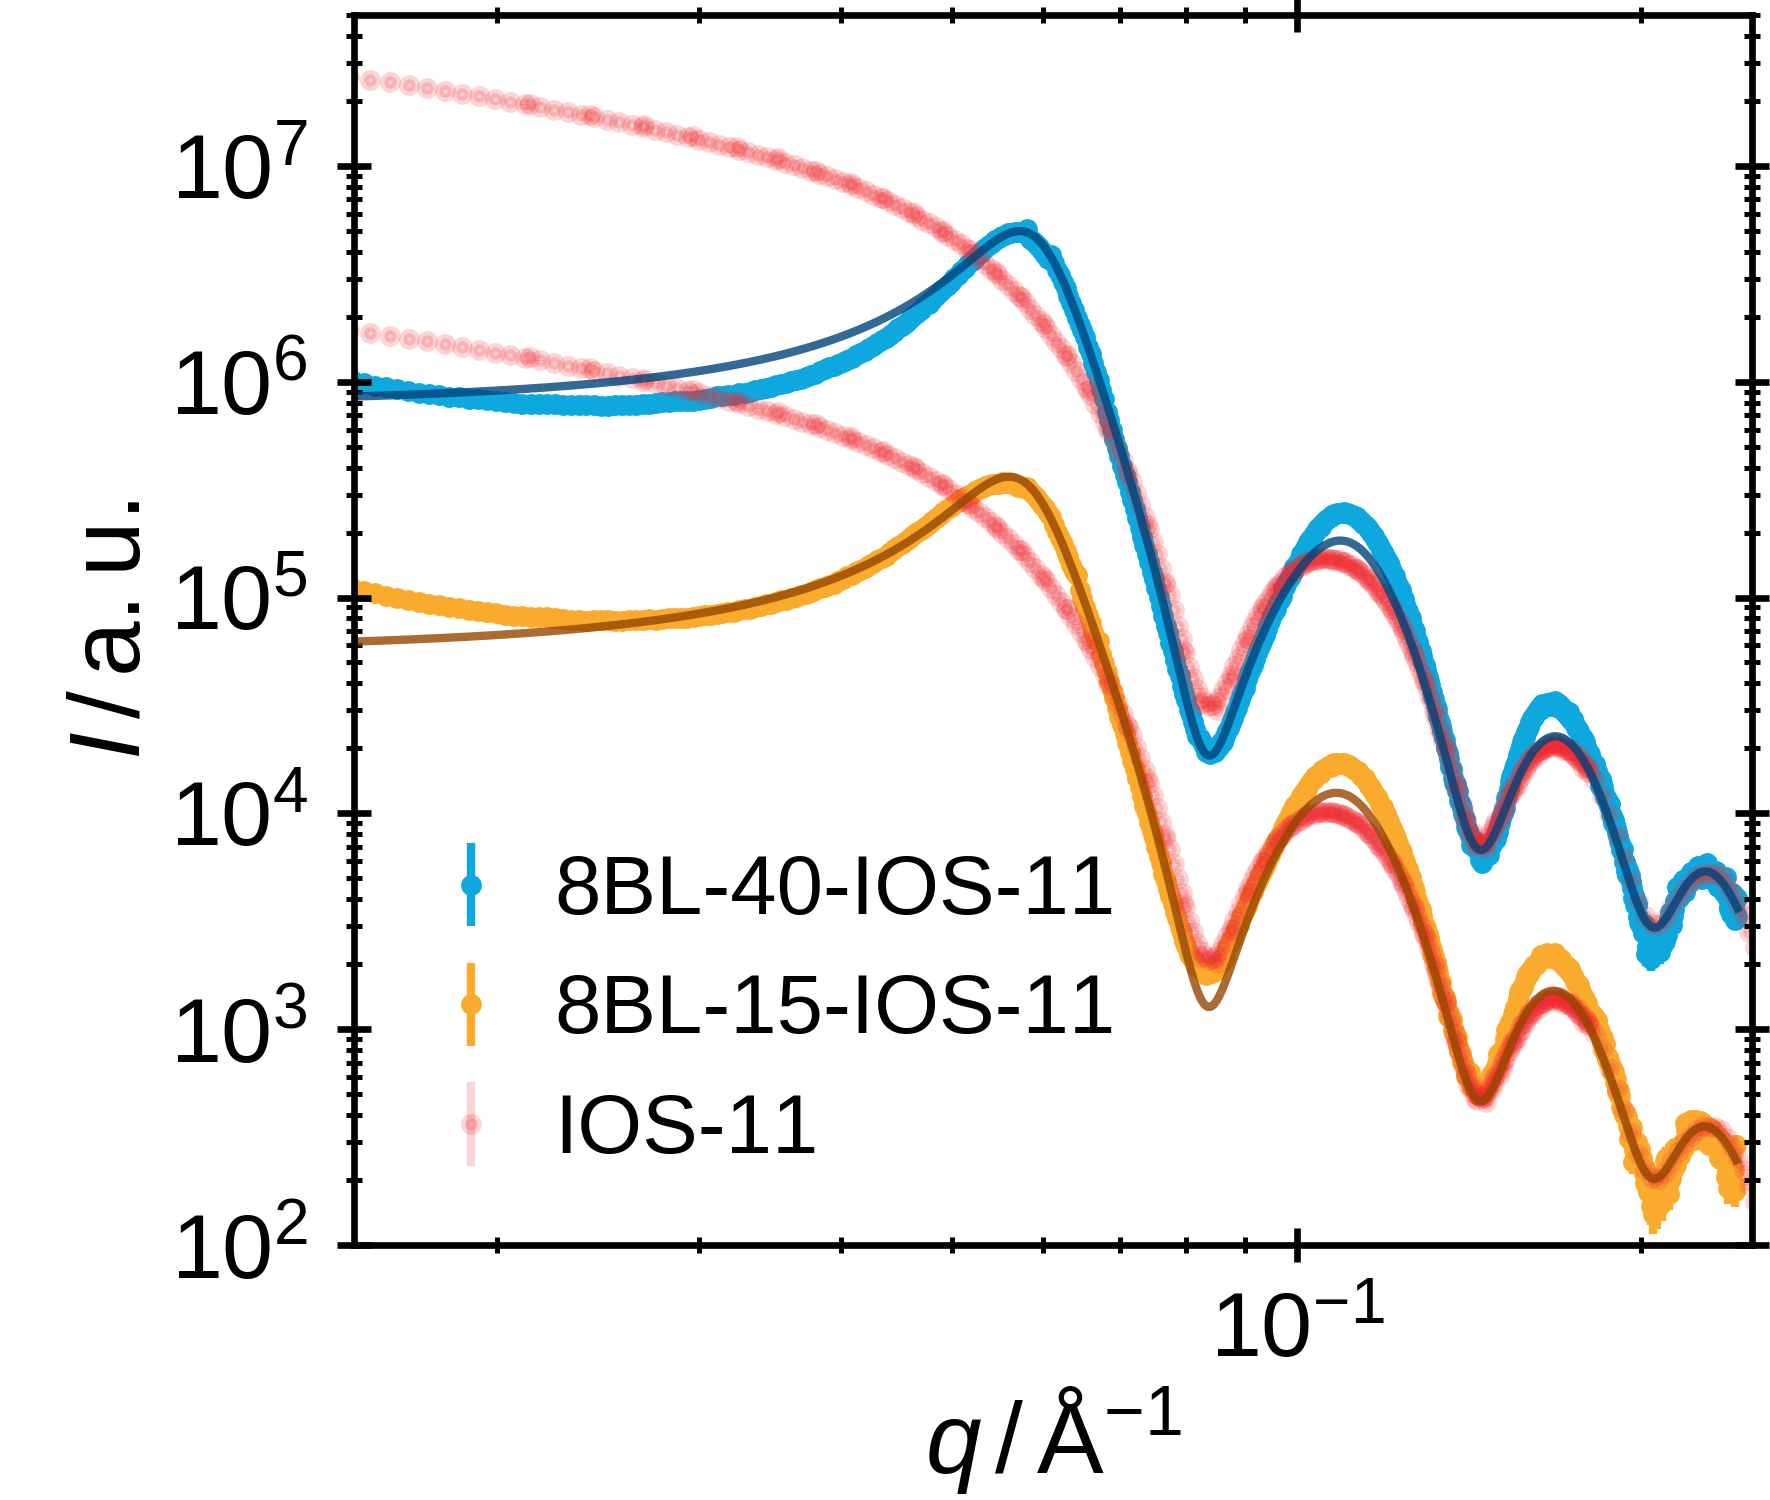
\includegraphics{looselyPackedNP_GISAXS_StructureFactor_8BL-x-IOS-11}
    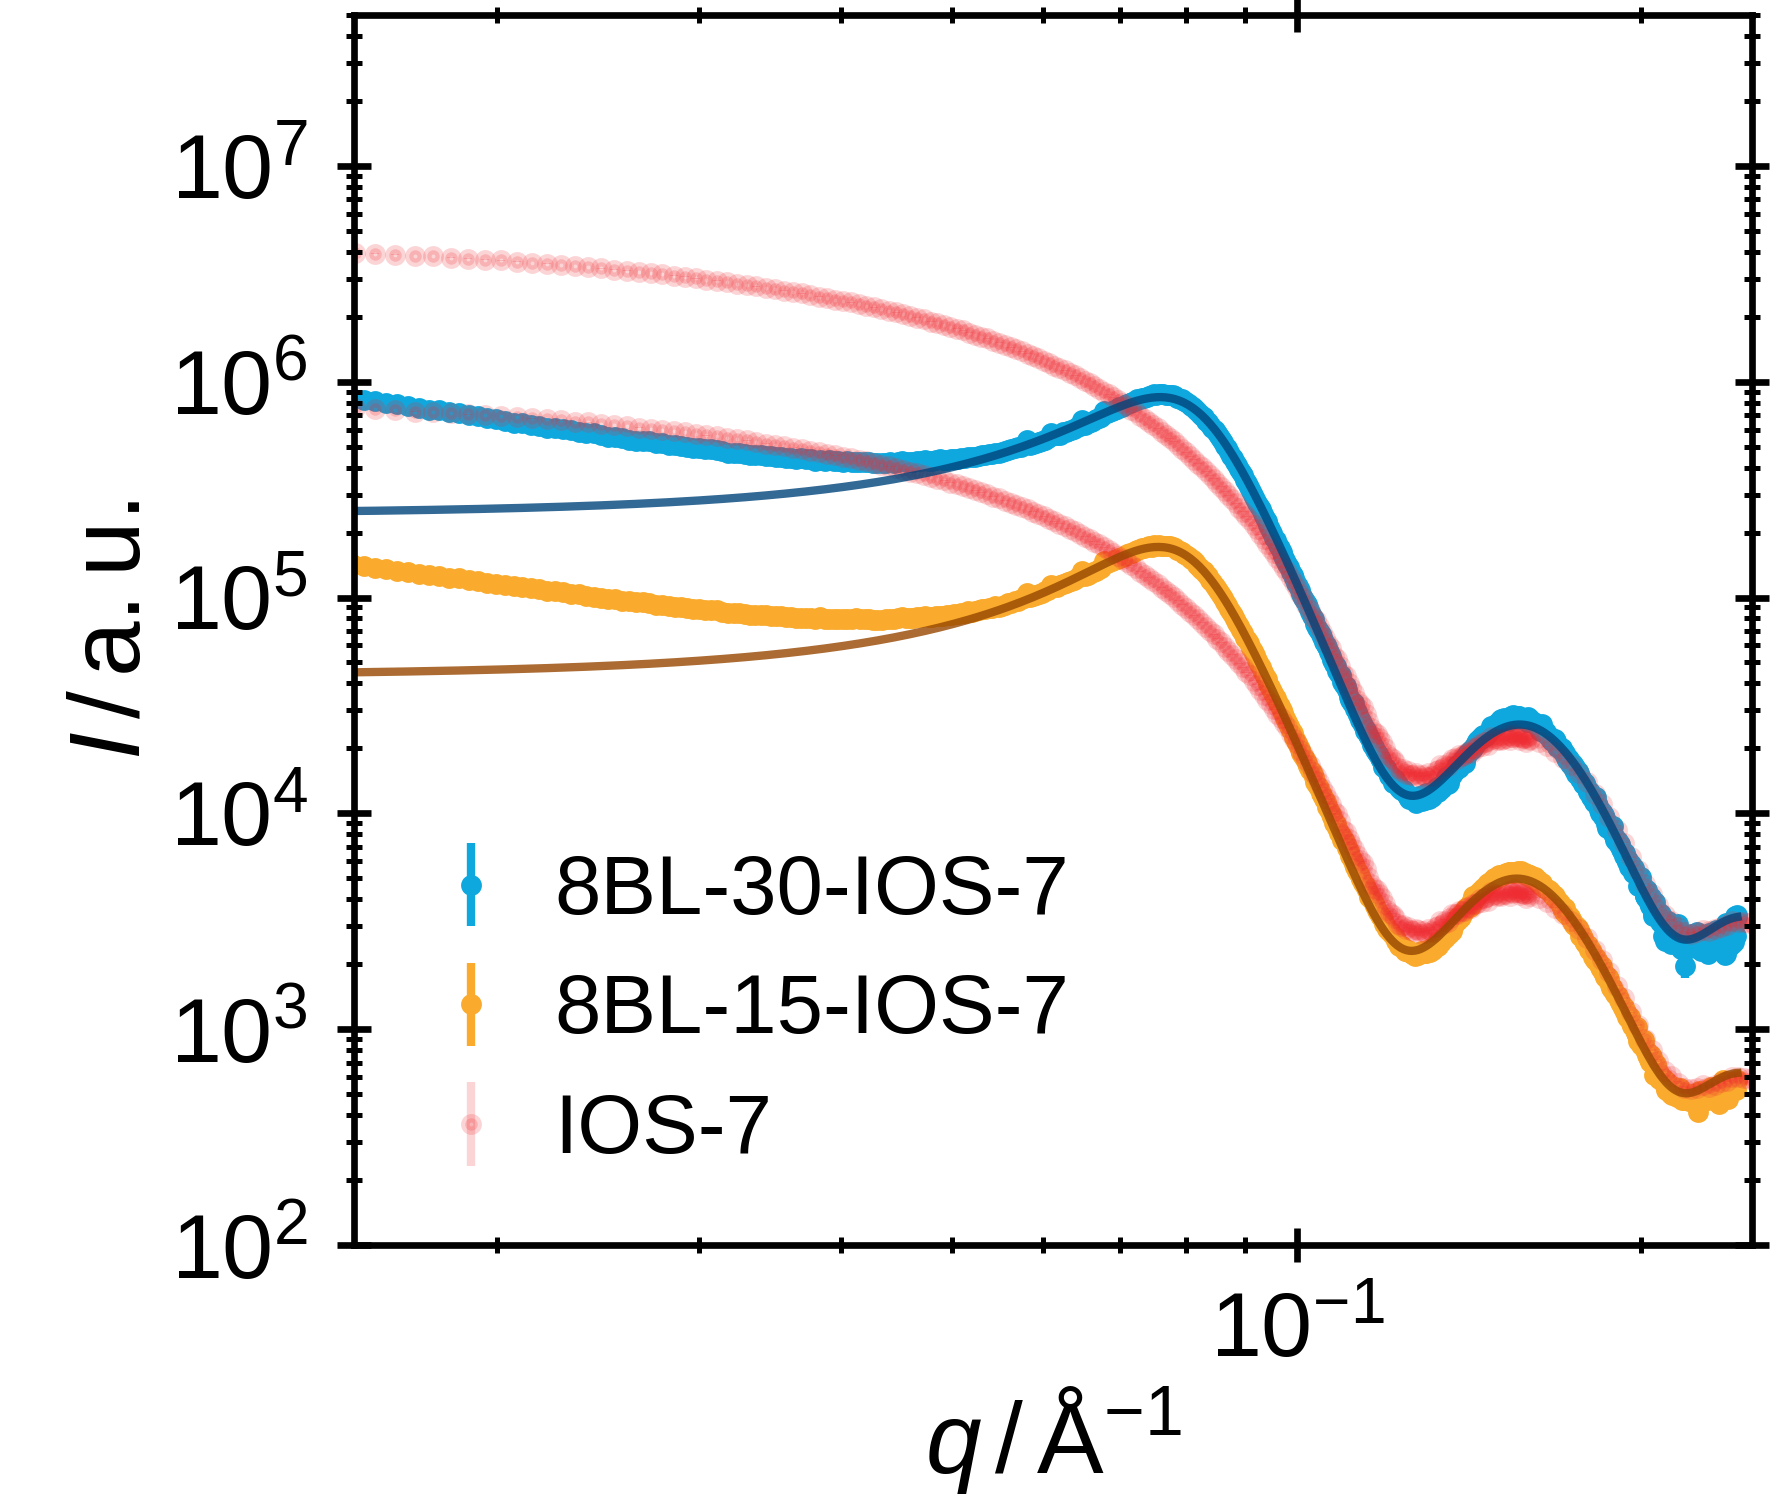
\includegraphics{looselyPackedNP_GISAXS_StructureFactor_8BL-x-IOS-7}
    \caption{\label{fig:looselyPackedNP:bilayerStacks:gisaxsHardSphereSF}Hard-sphere liquid structure factor in Percus-Yevick approximation fit to the data in the Yoneda band for the bilayer stack samples.}
  \end{figure}

  A hard-sphere radius of $5.708(6) \unit{nm}$ and $5.625(8) \unit{nm}$ is observed for 8BL-15-IOS-11 and 8BL-40-IOS-11, respectively, which is in comparable order of magnitude to the single spin-coated layers in \refsec{sec:looselyPackedNS:layers:gisaxs}, where a hard-sphere radius of $5.655(2) \unit{nm}$ is obtained.
  The packing fraction of $42.28(1) \%$ and $43.19(2) \%$ is also close to the value of $43.88 \%$ observed for SC-IOS-11.
  Similarly a hard-sphere radius of $3.976(2) \unit{nm}$ and $3.912(2) \unit{nm}$ and a packing fraction of $35.80(5)\%$ and $35.05(5) \%$ is obtained for 8BL-15-IOS-7 and 8BL-30-IOS-7, respectively.
  This is comparable to the $3.872(4) \unit{nm}$ and $34.20(9) \%$ obtained for SC-IOS-7.
  Therefore, it can be concluded that the nanospheres pack in a similar loose packing in the respective layers.
  However, due to the complex structure of the samples and the involved large length scales of the multilayered structures, further information about the bilayer structure are not accessible from GISAXS in this case.
\end{document}